\subsection{Performance Comparisons}
\label{sec:performance}
In Table \ref{table:performance}, \textit{FastEnhancer}-B outperforms all baseline models on almost every metric. While having relatively large number of parameters and MACs, its speed-optimized architecture results in the lowest RTFs. Our smallest model, \textit{FastEnhancer}-T, achieves remarkably low RTFs of 0.012 on Xeon and 0.013 on M1 while maintaining comparable performance to baseline models. As the model size increases, overall performance improves at the cost of increased latency. As a side observation, compared to \textit{FastEnhancer}-S, \textit{FastEnhancer}-M shows slightly degraded DNSMOS scores despite improved scores on every other metric. This indicates that relying on a limited set of objective metrics can lead to misleading conclusions.

\subsection{Ablation Studies}
\label{sec:ablation}
We performed ablation studies to validate the effectiveness of our architectural design. First, we explored the impact of convolution kernel size. Starting with \textit{FastEnhancer}-B, we modified every convolution whose frequency-axis kernel size is 3 in encoder and decoder blocks, enlarging their time-axis kernel size from 1 to 3.
This necessitated caching operations and significantly increased RTFs, but no improvement in quality or intelligibility was observed (Table \ref{table:ablation}).

Second, to investigate the effect of normalization layers, we replaced all BNs with LNs. While this maintained speech quality and intelligibility, it increased RTFs, despite having the same number of parameters and MACs. This result confirms that using BNs and fusing them into adjacent layers is the most efficient option.

Third, we created Dual-Path RNNs by replacing the frequency-axis MHSA blocks with frequency-axis GRU blocks.
While STOI scores were similar, DPRNNs clearly degraded SISDR compared to the proposed RNNFormers (Fig. \ref{fig:ablation}).
%Due to the page limit, we only include two metrics, but the tendencies were similar across other metrics.
% We deduce that since frequency RNN processes frequency bands sequentially, it requires more computational resources to achieve performance similar to a frequency transformer.
This demonstrates the superiority of self-attention over a recurrent approach for frequency modeling.

\begin{figure}[tp]
    \centerline{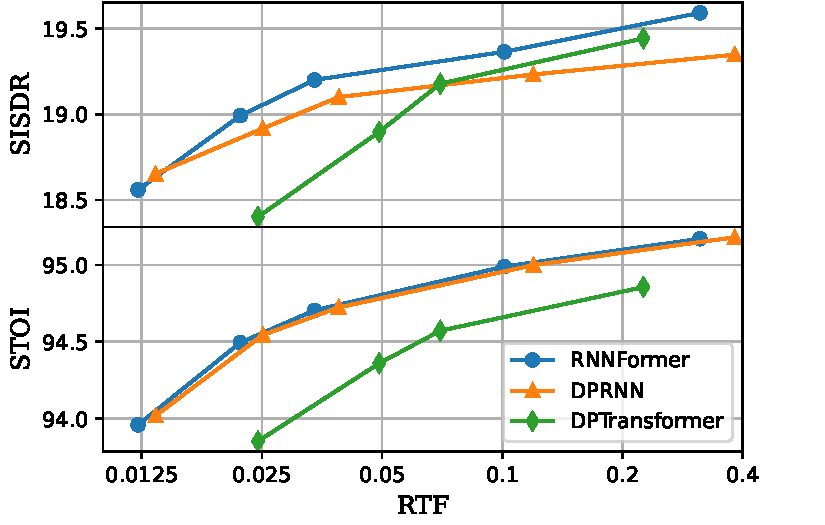
\includegraphics[width=1.0\linewidth]{fig_ablation.pdf}}
    \vspace{-0.4cm}
    \caption{Ablation study for RNNFormer.}
    \label{fig:ablation}
\end{figure}

Finally, we constructed Dual-Path Transformers by replacing the time-axis GRU blocks with time-axis MHSA blocks with a look-behind of 31 frames (corresponding to 0.5 seconds). Although DPTs have fewer parameters than RNNFormers, they require key-value caching, resulting in significantly increased RTFs. This result suggests that a recurrent approach is a more efficient choice than self-attention for temporal modeling in a streaming scenario.
